%
% File: chap01.tex
%
\let\textcircled=\pgftextcircled
\chapter{Flux in the core}
\label{chap:intro}

\initial{S}everal exercises from the book written by M. M. El Wakil~\cite{book01} are tackled in this homework. The problems in this section relate mostly to the third chapter of the book, covering the subject of the neutron flux distribution in cores.

%=======
\section{Finite cylinder}
\label{prob31}

\subsection{Problem}
\textit{Find the flux in a finite cylinder of radius $R$ and height $H$ using the diffusion theory.}

\subsection{Solution}

The diffusion equation can be written following Equation~\ref{eq31}.

\begin{equation}\label{eq31}
\nabla^2 \phi + B^2\phi = 0
\end{equation}

In a cylindrical coordinates system, the Laplacian $\nabla$ can be explicited according to Equation~\ref{eq32}.

\begin{equation}\label{eq32}
\nabla^2 \phi = \frac{\partial^2}{\partial r^2} + \frac{1}{r}\frac{\partial}{\partial r} + \frac{\partial^2}{\partial z^2}
\end{equation}

Consequently, we can rewrite Equation~\ref{eq31} to obtain Equation~\ref{eq33}.


\begin{equation}\label{eq33}
\frac{\partial^2 \phi(r, z)}{\partial r^2} + \frac{1}{r}\frac{\partial \phi(r, z)}{\partial r} + \frac{\partial^2 \phi(r, z)}{\partial z^2} + B^2\phi(r, z) = 0
\end{equation}

In order to solve this differential equation, one assumes that the axial flux component is independent from the radial flux component. In this case, the variables can be separated, using Definition~\ref{eq34}.


\begin{equation}\label{eq34}
\phi(r, z) = \rho(r)\zeta(z)
\end{equation}

This implies Equation~\ref{eq35}.


\begin{equation}\label{eq35}
\zeta(z)\frac{\partial^2 \rho(r)}{\partial r^2} + \frac{\zeta(z)}{r}\frac{\partial \rho(r)}{\partial r} + \rho(r)\frac{\partial^2 \zeta(z)}{\partial z^2} + B^2\rho(r)\zeta(z) = 0
\end{equation}

Now, it is useful to divide the equation by $\rho(r)\zeta(z)$ in order to isolate the $r$-component from the $z$-component, as seen in Equation~\ref{eq36}.


\begin{equation}\label{eq36}
\frac{1}{\rho(r)}\frac{\partial^2 \rho(r)}{\partial r^2} + \frac{1}{r\rho(r)}\frac{\partial \rho(r)}{\partial r} + \frac{1}{\zeta(z)}\frac{\partial^2 \zeta(z)}{\partial z^2} = -B^2
\end{equation}

Now, we have an equation of the form $f(x) + g(y) = cst$. This equation can only be verified if $f(x) = cst$ and $g(y) = cst$. Consequently, we have the following system of equations~\ref{eq37} and~\ref{eq38} to solve.

\begin{alignat}{2}
\frac{1}{\rho(r)}\frac{\partial^2 \rho(r)}{\partial r^2} + \frac{1}{r\rho(r)}\frac{\partial \rho(r)}{\partial r} = -\alpha \label{eq37} \\     \frac{1}{\zeta(z)}\frac{\partial^2 \zeta(z)}{\partial z^2} = -\beta \label{eq38}
\end{alignat}

Where:

\begin{conditions}
\alpha + \beta & $B^2$
\end{conditions}

Focusing on Equation~\ref{eq37} first, one can multiply both sides by $\rho(r)$, obtaining Equation~\ref{eq39}.

\begin{equation}\label{eq39}
\frac{\partial^2 \rho(r)}{\partial r^2} + \frac{1}{r}\frac{\partial \rho(r)}{\partial r} + \alpha\rho(r) = 0
\end{equation}

Equation~\ref{eq39} is known as a Bessel equation. The solutions to this equation are the first and second kind of Bessel functions, $J_0(\sqrt{\alpha}r)$ (Figure~\ref{fig31}) and $Y_0(\sqrt{\alpha}r)$ (Figure~\ref{fig32}).

\begin{figure}[t!]
	\centering
	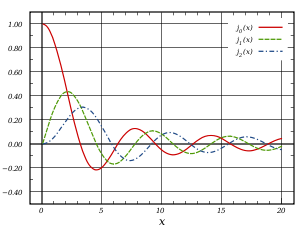
\includegraphics[height=0.3\textheight]{fig/bessel_j.png}
	\mycaption[Bessel function of the first kind - $J$]{Bessel function of the first kind - $J$.}
	\label{fig31}
\end{figure}


\begin{figure}[t!]
	\centering
	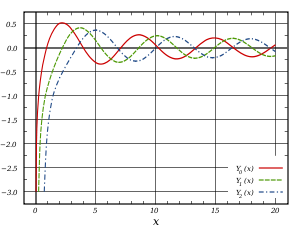
\includegraphics[height=0.3\textheight]{fig/bessel_y.png}
	\mycaption[Bessel function of the second kind - $Y$]{Bessel function of the second kind - $Y$.}
	\label{fig32}
\end{figure}

Consequently, the solution will be of the form $\rho(r) = AJ_0(\sqrt{\alpha}r) + CY_0(\sqrt{\alpha}r)$, $A$ and $C$ being constants.

We can now use boundary conditions. We know that the radial component of the flux has to be greater or equal to 0 $\forall r$. In our system, r = 0 at the center of the cylinder. However, $\lim_{r\to 0} Y_0(r) = -\infty$, implying that $C = 0$.

We also know that at a radius $R_e = R + \delta_e$, the flux is to be zero. Thus, $\phi(R_e) = 0$. So, we have to solve Equation~\ref{eq310}.

\begin{equation}\label{eq310}
AJ_0(\sqrt{\alpha}R_e) = 0
\end{equation}

This can be solved by A = 0, in which case we would obtain the trivial solution $\rho(r) = 0$, of no interest. $J_0(x) = 0$ can be verified for several $x$. However, since the flux has to be positive, the solution has to be the first zero of the function, happening for $x = 2.405$. Hence, Equation~\ref{eq310} is verified for $\sqrt{\alpha}R_e = 2.405$.

Thus, we have the solution of the radial component of the flux, presented in Equation~\ref{eq311}.

\begin{equation}\label{eq311}
\rho(r) = AJ_0(\frac{2.405}{R_e}r)
\end{equation}

Now, we can focus on the axial component of the flux, shown in Equation~\ref{eq38}. It is interesting to recognize in this equation the equation for an infinite slab geometry, for which the solution is known, explicited in Equation~\ref{eq312}.

\begin{equation}\label{eq312}
\zeta(z) = D\cos(\frac{\pi}{H_e}z)
\end{equation}

Finally, one can compute the flux $\phi(r, z)$, according to Equation~\ref{eq313}.

\begin{equation}\label{eq313}
\phi(r, z) = \phi_0 * J_0(\frac{2.405}{R_e}r)\cos(\frac{\pi}{H_e}z)
\end{equation}

Where $\phi_0 = A * D$.

We can also deduce the buckling $B^2 = \alpha + \beta = \left( \frac{2.405}{R_e} \right)^2 + \left( \frac{\pi}{H_e} \right)^2$.

\section{Radioactivity}
\label{prob32}

\subsection{Problem}
\textit{A radioactive sample is composed of two independently radioactive isotopes. A nuclear counter whose output is directly proportional to the total activity of the sample was used and gave the following count (Table 1-13,~\cite{book01}). Find the half-life and the decay constant of each of the two isotopes.}

\subsection{Solution}

The sample is composed of two independently radioactive isotopes. We assume that their respective hal-life is sufficiently different and low for one isotope contribution to be neglected after 26 hours. This means that after 26h, only one isotope, B, is contributing, as seen in Equation~\ref{eq314}.

\begin{equation}\label{eq314}
A(t) = A_{B, 0}e^{-\lambda_B t}
\end{equation}

Assuming that after 26 hours, the contribution comes only from isotope A. This implies that we can use the data points t=26h and t=28h to obtain a system of equation. This system is needed to solve for $A_{B, 0}$ and for $\lambda_B$.

We can write Equations~\ref{eq315} and~\ref{eq316}.


\begin{equation}\label{eq315}
\lambda_B = \frac{\ln(1072/1010)}{3600 * (28-26)} = \text{\num{8.2744e-6}}
\end{equation}

\begin{equation}\label{eq316}
A_{B,0} = 1010 * e^{\lambda_B (28*3600)} = 842.4
\end{equation}

Consequently, the half-life of isotope B is $T_{1/2, B} = 23.27h$.

Substituting the activity due to isotope B from the total measured, we can obtain the contribution of isotope C. Hence, $A(C, t=0) = 102000-842.4 = 101157.6$ and $A(C, t=4) = 26300 - A_{B, 0}e^{-\lambda_B 4*3600} = 25552$.

Hence, using Equation~\ref{eq317}, we can obtain.


\begin{equation}\label{eq317}
A(t) = A_{C, 0}e^{-\lambda_C t}
\end{equation}

And so,

\begin{equation}\label{eq318}
\lambda_C = \frac{\ln(101157.6/25552)}{3600 * 4} = \text{\num{9.555e-5}}
\end{equation}


Consequently, the half-life of isotope C is $T_{1/2, C} = 2.015h$. We can verify that after 10 periods of isotopes C half-life (21h), only the contribution of isotope B would remain. The calculation thus stands.

\section{Thermal fission factor}
\label{prob33}

\subsection{Problem}
\textit{Calculate the thermal-fission factor for 2200-m/sec neutrons for (a) natural uranium and for (b) 2 percent, (c) 20 percent, and (d) fully enriched uranium.}

\subsection{Solution}

The thermal fission factor, $\eta$, is described using Equation~\ref{eq319}.

\begin{equation}\label{eq319}
\eta = \frac{\nu\Sigma_f}{\Sigma_f + \Sigma_c} = \nu\frac{N_5\sigma_f^5}{N_5\sigma_f^5 + N_5\sigma_c^5 + N_8\sigma_c^8}
\end{equation}

Where:

\begin{conditions}
N_5 & Density of $U^{235}$ \\
N_8 & Density of $U^{238}$ \\
\sigma_f^5 & microscopic fission cross section of $U^{235}$ \\
\sigma_c^5 & microscopic capture cross section of $U^{235}$ \\
\sigma_c^8 & microscopic capture cross section of $U^{238}$
\end{conditions}

Knowing that the enrichment can be written $e = \frac{N_5}{N_5 + N_8}$, one can rewrite Equation~\ref{eq319} into Equation~\ref{eq320}.


\begin{equation}\label{eq319}
\eta = \nu\frac{e\sigma_f^5}{e\sigma_f^5 + e\sigma_c^5 + (1-e)\sigma_c^8}
\end{equation}


Considering $\nu = 2.43$, $\sigma_f^5 = 571.1\ b$, $\sigma_a^5 = \sigma_c^5 + \sigma_f^5 = 678.2\ b$ and $\sigma_c^8 = 2.73\ b$, the answers to \textit{(a), (b), (c)} and \textit{(d)} are respectively $1.30$, $1.71$,  $2.01$ and $2.05$.

\section{Cubical reactor core}
\label{prob34}

\subsection{Problem}
\textit{The extrapolation lengths in a cubical reactor core are negligibly small. Find the ratio of average to maximum flux if the flux distribution is:
(a) Sinusoidal in the x, y and z directions
(b) Sinusoidal in the x and y directions but uniform in the z direction
(c) Sinusoidal in the x direction only and uniform in the y and z directions.}

\subsection{Solution}

The average flux is given by Equation~\ref{eq326}.

\begin{equation}\label{eq326}
\overline{\phi} = \frac{\iiint_V \phi(x,y,z) \,dx\,dy\,dz}{V}
\end{equation}

If we consider a flux sinusoidal in the x, y and z directions, then we have~\ref{eq327}, considering $a$ the side of the cube.

\begin{equation}\label{eq327}
\phi(x,y,z) = \phi_0\cos(\frac{\pi x}{a})\cos(\frac{\pi y}{a})\cos(\frac{\pi z}{a})
\end{equation}

The flux being maximum at the center of the cube, the integration has to be done from 0 to $a/2$. The triple integrals are independent from one another, and thus we can write Equation~\ref{eq328}.

\begin{equation}\label{eq328}
\overline{\phi(x,y,z)} = \frac{\phi_0}{V} \int_0^{a/2} \cos(\frac{\pi x}{a}) \,dx \int_0^{a/2} \cos(\frac{\pi y}{a}) \,dy \int_0^{a/2} \cos(\frac{\pi z}{a}) \,dz 
\end{equation}


Knowing Equation~\ref{eq331}, we can obtain Equation~\ref{eq329}.

\begin{equation}\label{eq331}
\int_0^{a/2} \cos(\frac{\pi x}{a}) \,dx = \left[ \frac{a \sin(\frac{\pi x}{a})}{\pi} \right]_0^{a/2} = \frac{a}{\pi}
\end{equation}

\begin{equation}\label{eq329}
\overline{\phi(x,y,z)} = \frac{\phi_0 a^3}{V\pi^3} 
\end{equation}

The maximum flux being $\phi_0$, the ratio of average to maximum flux is equal to $\frac{a^3}{V\pi^3}$. V being $a^3$, it is easy to see that the ratio is $\frac{1}{\pi^3}$.

Now, if we consider a flux sinusoidal in the x and y directions but uniform in the z direction, we can write Equation~\ref{eq328} as Equation~\ref{eq330}.


\begin{equation}\label{eq330}
\overline{\phi(x,y,z)} = \frac{\phi_0}{V} \int_0^{a/2} \cos(\frac{\pi x}{a}) \,dx \int_0^{a/2} \cos(\frac{\pi y}{a}) \,dy \int_0^{a/2} B \,dz 
\end{equation}

Knowing Equation~\ref{eq331} and Equation~\ref{eq332}, we can write Equation~\ref{eq333}.

\begin{equation}\label{eq332}
\int_0^{a/2} B \,dx = \left[ Bx + C \right]_0^{a/2} = \frac{Ba}{2}
\end{equation}

\begin{equation}\label{eq333}
\overline{\phi(x,y,z)} = \frac{\phi_0 B a^3}{2 V\pi^2} 
\end{equation}

And thus, the ratio of average to maximum flux is equal to $\frac{B}{2 \pi^2}$.

Finally, using the same reasoning, we can obtain Equation~\ref{eq334} for the last case (uniform flux B and C for y and z directions respectively).

\begin{equation}\label{eq333}
\frac{\overline{\phi(x,y,z)}}{\phi_{max}} = \frac{B C}{4 \pi} 
\end{equation}

\section{Nuclear temperature coefficient}
\label{prob35}

\subsection{Problem}
\textit{Assuming constant $k_{\infty}$ and $B^2$, and a $1/V$ dependence of the thermal neutron absorption, show that the nuclear temperature coefficient in a thermal reactor is given by $\frac{\delta\rho_n}{\delta T} = - \frac{B^2 L^2}{2k_{\infty}T}$.}

\subsection{Solution}

We know that $L=\sqrt{\frac{d}{\Sigma_a}}$ and that $D = \frac{\lambda_{tr}}{3}$.

Consequently,

\begin{equation}\label{eq320}
L^2 = \frac{\lambda_a\lambda_{tr}}{3} = \frac{1}{3\Sigma_a\Sigma_s}
\end{equation}

In the $1/v$ region, v is proportional to $\sqrt{T}$. Consequently, $\sigma_a = \sigma_{a,0}\sqrt{\frac{T_0}{T}}$.

So, we can write $L^2 = L_0^2\sqrt{\frac{T_0}{T}}$.

Now, we can start from Equation~\ref{eq321}.


\begin{equation}\label{eq321}
k_{eff} = \frac{k_{\infty} l_f}{1 + L^2B^2}
\end{equation}

Knowing that $\rho = \frac{k_{eff} - 1}{k_{eff}}$, one can write:


\begin{equation}\label{eq322}
\rho = \frac{k_{\infty} - 1 - L^2B^2}{k_{\infty}}
\end{equation}

And so, plugging in $L^2$:


\begin{equation}\label{eq323}
\rho = \frac{k_{\infty} - 1}{k_{\infty}} - \frac{B^2L_0^2\sqrt{\frac{T}{T_0}}}{k_{\infty}}
\end{equation}

Derivative of this equation with regards to $T$ gives us:


\begin{equation}\label{eq324}
\frac{\delta \rho}{\delta T} = - \frac{B^2L_0^2(T T_0)^{-1/2}}{2k_{\infty}}
\end{equation}

The temperature coefficient at T is given for $T=T_0$, in which case:


\begin{equation}\label{eq325}
\frac{\delta \rho}{\delta T} = - \frac{B^2L^2}{2k_{\infty}T}
\end{equation}

\section{Spherical reactor}
\label{prob36}

\subsection{Problem}
\textit{Solve the diffusion equation ($\nabla^2 \phi + B^2\phi = 0$) for a bare spherical core of radius $R$ and extrapolated radius $R_e$.}

\subsection{Solution}

The spherical diffusion equation can be written using Equation~\ref{eq334}.


\begin{equation}\label{eq334}
\frac{\partial^2 \phi(r)}{\partial r^2} + \frac{2}{r}\frac{\partial \phi(r)}{\partial r} + B^2\phi(r) = 0
\end{equation}

Using the substitution $\phi(r) = \frac{\Phi(r)}{r}$, as well as the product rule for the first derivative, shown in Equation~\ref{eq3351} and for the second derivative, shown in Equation~\ref{eq3352}, we can obtain Equation~\ref{eq335}.


\begin{equation}\label{eq3351}
\frac{\partial f(r)g(r)}{\partial r} = f'(r)g(r) + f(r)g'(r)
\end{equation}

\begin{equation}\label{eq3352}
\frac{\partial^2 f(r)g(r)}{\partial r^2} = f''(r)g(r) + 2f'(r)g'(r) + f(r)g''(r)
\end{equation}

In our case, $f(r) = \frac{1}{r}$ and $g(r) = \Phi(r)$.

\begin{equation}\label{eq335}
\frac{2}{r^3}\Phi(r) - \frac{2}{r^2}\frac{\partial \Phi(r)}{\partial r} + \frac{1}{r}\frac{\partial^2 \Phi(r)}{\partial r^2} - \frac{2}{r^3}\Phi(r) + \frac{2}{r^2}\frac{\partial \Phi(r)}{\partial r} + \frac{1}{r}B^2\Phi(r) = 0
\end{equation}

This equation can trivially be simplified to Equation~\ref{eq336}, by eliminating terms and multiplying both sides by $r$.

\begin{equation}\label{eq336}
\frac{\partial^2 \Phi(r)}{\partial r^2} + B^2\Phi(r) = 0
\end{equation}

Equation~\ref{eq336} is well known and has two possible solutions, $\sin(Br)$ and $\cos(Br)$. Consequently, $\Phi(r) = A\cos(Br) + C\sin(Br)$, and finally, $\phi(r) = \frac{A}{r}\cos(Br) + \frac{C}{r}\sin(Br)$.

The flux has to be finite for every $r$, including $r=0$. This allows us to eliminate the cosinus part of the equation, because $\lim_{r\to 0} \frac{A}{r}\cos(Br) = - \infty$. So, $A = 0$.

The solution is thus given by Equation~\ref{eq337}.

\begin{equation}\label{eq337}
\phi(r) = \frac{C}{r}\sin(Br)
\end{equation}

The flux has to be zero at a distance $R_e$. Consequently, $\frac{C}{R_e}\sin(BR_e) = 0$. This is possible if and only if $C = 0$ (trival zero solution) or $\sin(BR_e) = 0$. This is possible for $B = \frac{n\pi}{R_e}$, $n$ being an odd integer. The flux has to stay positive, and so only the first zero of the sinus function can be physically true, $n = 1$.

Finally, the flux in the spherical reactor is $\phi(r) = \frac{C}{r}\sin(\frac{\pi}{R_e}r)$.


\subsection{Problem}
\textit{Consider a cylindrical reactor core and assume that the neutron flux $\phi$ is rotationally symmetric. Assume that the extrapolation length is negligible. Let $I(y)$ be the average of the flux taken in the x direction. Verify the relations $I(y) = 2 \int_0^{(R^2-y^2)^{1/2}} \phi(r)dx = 2 \int_y^R \frac{\phi(r)rdr}{(r^2-y^2)^{1/2}}$ and $\phi(r) = -\frac{1}{\pi} \int_r^R \frac{dI(y)}{dy} \frac{dy}{(y^2-r^2)^{1/2}}$. Thus, I and $\phi$ form an integral transform pair.}

\subsection{Solution}

$I(y)$, the average of the flux taken in the x direction, can be written using Equation~\ref{eq338}.


\begin{equation}\label{eq338}
I(y) = \int_{-\infty}^{\infty} \phi(r) dx = 2 \int_{0}^{\infty} \phi(r) dx 
\end{equation}

Considering that $x^2 + y^2 = r^2$, we can trivially obtain $x = \sqrt{r^2 - y^2}$. The core is a cylinder of radius R, and the flux is zero outside the core. Consequently, we can write Equation~\ref{eq339}.


\begin{equation}\label{eq339}
I(y) = 2 \int_{0}^{\sqrt{R^2-y^2}} \phi(r) dx
\end{equation}

We can now change the variable, by knowing that $dx = \frac{rdr}{\sqrt{r^2 - y^2}}$. Additionally, for $x = 0$, we have $r^2 = y^2$ and thus $r=y$. We obtain Equation~\ref{eq340}, proving the first part of the problem.


\begin{equation}\label{eq340}
I(y) = 2 \int_{y}^{R} \frac{\phi(r)rdr}{\sqrt{r^2 - y^2}}
\end{equation}

Now, this integral can be integrated by parts, following Equation~\ref{eq341}.


\begin{equation}\label{eq341}
I(y) = 2 \int_{y}^{R} \phi(r) \frac{d \sqrt{r^2-y^2}}{dr}dr = -2 \int_{y}^{R} \frac{d\phi(r)}{dr} \sqrt{r^2-y^2}dr + \left[ 2\phi(r)\sqrt{r^2-y^2} \right]_y^R
\end{equation}

The boundary conditions state that when $r=y$, the second term is zero, and when $r=R$, the flux is zero by assumption. The second term thus nullify, and we are left with Eqaution~\ref{eq342}.


\begin{equation}\label{eq342}
I(y) = -2 \int_{y}^{R} \frac{d\phi(r)}{dr} \sqrt{r^2-y^2}dr
\end{equation}

Now, we can can get the derivative of $I(y)$ with respect to $y$, in order to plug in into the second relation to verify. This is given by Equation~\ref{eq343}.


\begin{equation}\label{eq343}
\frac{dI(y)}{dy} = 2y \int_{y}^{R} \frac{d\phi(r)}{dr} \frac{1}{\sqrt{r^2-y^2}}dr
\end{equation}

We have to verify Equation~\ref{eq344}.


\begin{equation}\label{eq344}
\phi(r) = -\frac{1}{\pi} \int_r^R \frac{dI(y)}{dy} \frac{dy}{(y^2-r^2)^{1/2}}
\end{equation}

Substituting in the derivative of $I(y)$, we obtain Equation~\ref{eq345} by using a dummy variable $s = r$.


\begin{equation}\label{eq345}
\phi(r) = -\frac{1}{\pi} \int_r^R \int_y^R \frac{d\phi(s)}{ds} \frac{1}{\sqrt{s^2-y^2}} ds \frac{2ydy}{\sqrt{y^2-r^2}}
\end{equation}

Interchanging the variables in the integrals, according to Equation~\ref{eq346}, we can get~\ref{eq347}.


\begin{equation}\label{eq346}
\int_r^R dy \int_y^R ds = \int_r^R ds \int_r^S dy
\end{equation}

\begin{equation}\label{eq347}
\phi(r) = -\frac{1}{\pi} \int_r^R \int_r^S \frac{2ydy}{\sqrt{(y^2-r^2)(s^2-y^2)}} \frac{d\phi(s)}{ds} ds 
\end{equation}

Now, we can look in more details at part of this equation, $\eta = \int_r^S \frac{2ydy}{\sqrt{(y^2-r^2)(s^2-y^2)}}$. If we let $u=y^2$ and thus $du = 2ydy$, we can compute Equation~\ref{eq348}.

\begin{equation}\label{eq348}
\eta = \int_{r^2}^{S^2} \frac{du}{\sqrt{(u-r^2)(s^2-u)}}
\end{equation}

Our goal now becomes to find an integral of the form $\int_0^1 t^{x-1} (1-t)^{y-1} dt$, since the solutions to this kind of integrals is well-known, the $\beta$-functions.

Let $v = u-r^2$, then $u = v+r^2$ and we can write Equation~\ref{eq349}.


\begin{equation}\label{eq349}
\eta = \int_{0}^{S^2-r^2} \frac{dv}{\sqrt{v(s^2-r^2-v)}} = \frac{1}{\sqrt{s^2 - r^2}} \int_{0}^{S^2-r^2} \frac{dv}{\sqrt{v} \sqrt{1 - \frac{v}{s^2-r^2}}}
\end{equation}

And finally, if we let $w = \frac{v}{s^2-r^2}$, we can obtain Equation~\ref{eq350}.


\begin{equation}\label{eq350}
\eta = \int_{0}^{1} \frac{dw}{\sqrt{w} \sqrt{1-w}} = \beta(1/2, 1/2)
\end{equation}

And knowing that $\beta(x, y) = \frac{\Gamma(x)\Gamma(y)}{\Gamma(x+y)}$, as well as $\Gamma(1/2) = \sqrt{\pi}$ and $\Gamma(1) = 0! = 1$, $\eta = \pi$.

Now, coming back to Equation~\ref{eq347}, and plugging in $\eta$, we can finally obtain Equation~\ref{eq351}.

\begin{equation}\label{eq351}
\phi(r) = - \int_r^R \frac{d\phi(s)}{ds} ds = \phi(r) - \phi(R) = \phi(r)
\end{equation}

We thus verify the relations.
